\section{Digital Library}
\label{sec:lib}
Shady websites have long managed to monetize free content downloads.
Below we detail the ways in which we can follow their example to provide free
access to papers and liberate the ACM reader from covetousness.

\subsection{Fake Download Buttons}
\label{sec:fake}

Fake download buttons are a staple of modern download websites. They really
class up the web. Reifying, elegizing, and idealizing nature, these abstract
forms  direct the downloader's attention away from the url
to the ad-serving service to which the button points. A deceptive
d\'{e}tournement, the placement of these blissed-out buttons
challenges browsers to consider whether they really want to download the paper.
They could, after all, choose to abandon their line of inquiry and instead
watch their field's evolution vicariously through mainstream media, which cuts
down on the ACM's hosting costs.

By allowing advertisers to buy space on our digital library with which to
create ads that look like download buttons, advertisers can deceive users into
clicking an ad.
The advertiser and the ACM both profit off of these deceptive ads as the user
is redirected to see the advertiser's product while the ACM gets the revenue
for an impression. Some regulators have questioned this practice. But we
believe it is a win-win-win for consumers \footnote{Gary Cohn, the director of
  the National Economic Council, stressed in an interview with \textit{The Wall
Street Journal} compared a website without fake-download buttons to the menu at
P.J. Bland's: ``This is like putting only health food on the menu, because
unhealthy food tastes good. But you still shouldn't eat it because you might
die younger." The menus of a free society, in his reckoning, should include
both unhealthy and healthy items, and they should be labeled and priced
identically. It should be impossible for consumers to access independent,
third-party statistics about menu items. ``We believe our customers are
informed and engaged, and we trust that they are smart enough to make the
decisions that are right for them. We don't want the government treating them
like dotards," Gary Cohn said while spraying an unlabeled can of spray cheese
into his mouth.}.


Additionally, these download buttons could be functional in that they download
\textit{something}, but the ACM digital library will not impose any
restrictions on what may be downloaded from these fake buttons.
Therefore, advertisers are welcome to serve us infected PDFs or straight up
executables.
It is our position that users must be intelligent enough to hunt down the
proper download button, and that academics can learn valuable security
practices when they know that others could steal their research through
malicious downloads on the digital library.

To subvert ad blockers, the ad content will be natively hosted on the ACM
digital library as well.
Therefore, ad blockers will be unable to determine which requests are ad-related.

Additionally, we are revolutionizing the fake download practice by dynamically
randomizing the position of the actual download button.
Like serving ad content natively, this will make ad blockers functionally
useless as there will be no way to differentiate between ad content and ACM
content, providing users with instruction on the contingency of fate.
Moreover, this randomization makes it much harder for the user to learn the
positioning of the ads and therefore we hope to drive more clicks to our ad
partners and generate more revenue for the ACM.

Lastly, we are working on a proposal that will greatly reduce ACM hosting
costs, namely we  will replace the only real download button with a fake one.

\subsection{Rate-Limited Free Downloads}
\label{sec:limit}
Free download sites figured out long ago that you can make people pay for an
otherwise free product by making the process of obtaining that free product
difficult.
Therefore, we will split our digital library downloads into two tiers, the free
tier and the \premium tier.

The free tier will only allow downloads at slow speeds and no more than one
paper per day.
Additionally, the user will be required to stare at a screen compelling them to
upgrade while a counter decrements for 10 minutes before the download button is
clickable.
If the engagement of the user---monitored via gaze tracker and wearable
heart-rate monitor---falls below the Zone of Synergy\texttrademark, the counter will be restarted.
The \premium tier will allow unlimited downloads along with an upgraded
experience: the countdown clock will have ads replaced by a sponsored message
thanking you for upgrading and will feature a \premium digital clock face.

\subsection{Outsourced Captchas}
When a user requests a paper download, they will be required to submit a
captcha.
While many websites use captcha to prevent automated abuse, we see an
opportunity to profit.
We provide an API to botnets with which they may submit captchas to be
displayed to users attempting to download files.
Their responses to these captchas are sent back to the botnet thus allowing the
botnet to proceed with whatever attack the captcha was preventing.
We believe we can sell this human captcha solving service for a few cents per
captcha.

Users will not question the presence of captchas on the digital
library as they have already been conditioned to fill captchas for all sorts of
free services.
As such, we do not believe that our user base will know that the ACM is
slinging captcha solutions on the side.

\subsection{ACM Digital Library Toolbar}
Every ACM paper will be distributed as an executable.
Running this executable will ``install" the paper to the user's desktop.
The only purpose of the install is to push the ACM Digital Library toolbar on
the user.
While the toolbar itself is optional, its installation is opt-out.
The ACM Digital Library toolbar will be installed for the user's web browsers where it
will follow them from site to site collecting information about their browsing
habits.
We will provide this information to our partners for a nominal fee who may use
this user data to curate a product-based lifestyle that will make our readers' lives
more relevant to advertisers.

Additionally, the toolbar will constantly mine bitcoins on the user's machine
and send the mined coins to the ACM's wallet.
If the user has a GPU, the development drivers will be silently installed along
with the toolbar to enable GPU mining.
We hope that one day the ACM mining pool becomes so large that we become a
dominant player in the Bitcoin economy.
If we ever reach a simple majority of the mining power, we WILL mount a 51\%
attack to seize control of the network for our own financial gain.

In order to comply with New Jersey's backwards laws about involuntary Bitcoin
mining \cite{tidbit}, all New Jersey residents will be preemptively banned from
the ACM Digital Library and the greater academic community.

\subsection{Impact Factometer}

Researchers want their projects to have meaning and impact. Administrators like to market their department's product as meaningful and impactful. But how can researchers tell their work is saving the world?

Simple. Once a quarter, the Ricketts family convokes Gary Cohn, Dennis Rodman,
Colonel Sanders, and the rest of the Economic Advisory Council at Chicago's
historic Wrigley Field to make use of the stadium's native Noiseometer. As Pat
Hughes reads the papers over the PA , the council---taking especial care to
note the presence of key phrases like ``cross-promotional deal mechanics
revenue streams jargon synergy" and ``a strategic planning initiative\ldots
with a focus on strategic dynamism"---emits cheers in proportion to its
perception of the paper's impact, and these cheers are registered on the
Noiseometer, which assigns metrics of impact to each paper, as shown in Figure~\ref{fig:noiseometer}


\begin{figure}
  \centering
  %https://archive.org/details/414803main_0203243
  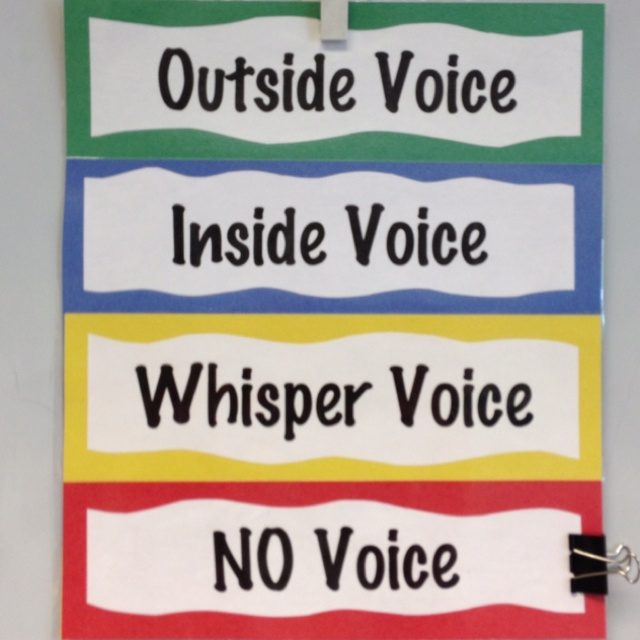
\includegraphics[width=0.45\textwidth]{figures/noiseometer.jpeg}
  \caption{A model-year 1985 Noiseometer, prized by collectors for its muted
  design that limns adumbrations of sound. The paper in which these meetings
were proposed was met at the first such convening of the Council with a cheer
so loud it registered a ``Nowhere Permissible Voice" \todo{maybe think of
something better} (not shown) on this scale.}
  \label{fig:noiseometer}
\end{figure}


These metrics empower our research partners to be certain their research is having a real-world impact.  It is important for researchers to know that they don't risk deactivation or exile if they remain on track.
